%-----------------------------------------------------------------------
%
%   UFRJ  - Universidade Federal do Rio de Janeiro
%   COPPE - Coordenação dos Programas de Pós-graduação em Engenharia
%   PEE   - Programa de Engenharia Elétrica
%
%
%   Projeto EMMA - 
%
%                                                        10/jul/15, Rio
%                                                        Ramon R. Costa
%----------------------------------------------------------------------
%
%  Compilar usando PDFLaTeX
%
%----------------------------------------------------------------------
\documentclass[12pt,a4paper]{article}
\usepackage{macros/ROSApackages} 

%-----------------------------------------------------------------------
%
%   UFRJ  - Universidade Federal do Rio de Janeiro
%   COPPE - Coordena��o dos Programas de P�s-gradua��o em Engenharia
%   PEE   - Programa de Engenharia El�trica
%
%
%   Projeto ROSA - Rob� para opera��o de stoplogs alagados
%
%   Settings
%                                                         Ramon R. Costa
%                                                         20/mar/14, Rio
%-----------------------------------------------------------------------

%---------------------------------------------------------- COLORS -----
%--------------------------------------------------- Bright colors -----
\definecolor{brightred}     {rgb}{1.00, 0.95, 0.95}
\definecolor{brightgreen}   {rgb}{0.95, 1.00, 0.95}
\definecolor{brightblue}    {rgb}{0.95, 0.95, 1.00}

\definecolor{brightyellow}  {rgb}{1.00, 1.00, 0.95}
\definecolor{brightmagenta} {rgb}{1.00, 0.95, 1.00}
\definecolor{brightcyan}    {rgb}{0.95, 1.00, 1.00}

\definecolor{brightorange}  {rgb}{1.00, 0.95, 0.85}

%----------------------------------------------------- Pale colors -----
\definecolor{palered}     {rgb}{1.00, 0.85, 0.85}
\definecolor{palegreen}   {rgb}{0.85, 1.00, 0.85}
\definecolor{paleblue}    {rgb}{0.85, 0.85, 1.00}

\definecolor{paleyellow}  {rgb}{1.00, 1.00, 0.85}
\definecolor{palemagenta} {rgb}{1.00, 0.85, 1.00}
\definecolor{palecyan}    {rgb}{0.85, 1.00, 1.00}

\definecolor{paleorange}  {rgb}{1.00, 0.85, 0.65}

%---------------------------------------------------- Light colors -----
\definecolor{lightred}     {rgb}{0.95, 0.00, 0.00}
\definecolor{lightgreen}   {rgb}{0.00, 0.95, 0.00}
\definecolor{lightblue}    {rgb}{0.00, 0.00, 0.95}

\definecolor{lightyellow}  {rgb}{0.95, 0.95, 0.00}
\definecolor{lightmagenta} {rgb}{0.95, 0.00, 0.95}
\definecolor{lightcyan}    {rgb}{0.00, 0.95, 0.95}

\definecolor{lightgray}    {rgb}{0.95, 0.95, 0.95}

\definecolor{lightorange}  {rgb}{0.95, 0.63, 0.00}

%--------------------------------------------------- Middle colors -----
\definecolor{midred}     {rgb}{0.85, 0.00, 0.00}
\definecolor{midgreen}   {rgb}{0.00, 0.85, 0.00}
\definecolor{midblue}    {rgb}{0.00, 0.00, 0.85}

\definecolor{midyellow}  {rgb}{0.85, 0.85, 0.00}
\definecolor{midmagenta} {rgb}{0.85, 0.00, 0.85}
\definecolor{midcyan}    {rgb}{0.00, 0.85, 0.85}

\definecolor{midgray}    {rgb}{0.85, 0.85, 0.85}

\definecolor{midorange}  {rgb}{0.85, 0.57, 0.00}

%--------------------------------------------------- Normal colors -----
\definecolor{red}     {rgb}{0.75, 0.00, 0.00}
\definecolor{green}   {rgb}{0.00, 0.75, 0.00}
\definecolor{blue}    {rgb}{0.00, 0.00, 0.75}

\definecolor{yellow}  {rgb}{0.75, 0.75, 0.00}
\definecolor{magenta} {rgb}{0.75, 0.00, 0.75}
\definecolor{cyan}    {rgb}{0.00, 0.75, 0.75}

\definecolor{gray}    {rgb}{0.75, 0.75, 0.75}

\definecolor{orange}  {rgb}{0.75, 0.50, 0.00}

%--------------------------------------------------- Shadow colors -----
\definecolor{shadred}     {rgb}{0.65, 0.00, 0.00}
\definecolor{shadgreen}   {rgb}{0.00, 0.65, 0.00}
\definecolor{shadblue}    {rgb}{0.00, 0.00, 0.65}

\definecolor{shadyellow}  {rgb}{0.65, 0.65, 0.00}
\definecolor{shadmagenta} {rgb}{0.65, 0.00, 0.65}
\definecolor{shadcyan}    {rgb}{0.00, 0.65, 0.65}

\definecolor{shadgray}    {rgb}{0.65, 0.65, 0.65}

\definecolor{shadorange}  {rgb}{0.65, 0.43, 0.00}

%--------------------------------------------------- Darker colors -----
\definecolor{darkred}     {rgb}{0.50, 0.00, 0.00}
\definecolor{darkgreen}   {rgb}{0.00, 0.50, 0.00}
\definecolor{darkblue}    {rgb}{0.00, 0.00, 0.50}

\definecolor{darkyellow}  {rgb}{0.50, 0.50, 0.00}
\definecolor{darkmagenta} {rgb}{0.50, 0.00, 0.50}
\definecolor{darkcyan}    {rgb}{0.00, 0.50, 0.50}

\definecolor{darkgray}    {rgb}{0.50, 0.50, 0.50}

\definecolor{darkorange}  {rgb}{0.50, 0.33, 0.00}

%-------------------------------------------------- Hyperref setup -----
\hypersetup{
  breaklinks   = true,
  colorlinks   = true,
  linkcolor    = darkblue,
  anchorcolor  = darkcyan,
  citecolor    = darkred,
  filecolor    = darkorange,
  menucolor    = darkmagenta,
  urlcolor     = darkgreen,
  pdfhighlight = /I,
  pdfstartview = FitH,
  pdfview      = FitH
}

%---------------------------------------------- DOCUMENT STRUCTURE -----

%------------------------------------------------- Page appearance -----
\setlength{\textheight    }{250mm}
\setlength{\textwidth     }{175mm}
\setlength{\footskip      }{10mm}
\setlength{\footnotesep   }{5mm}
\setlength{\headheight    }{10mm}
\setlength{\headsep       }{5mm}
\setlength{\oddsidemargin }{-6mm}
\setlength{\evensidemargin}{-6mm}
\setlength{\topmargin     }{-15.4mm}
\setlength{\marginparsep  }{0pt}
\setlength{\marginparwidth}{0pt}
\setlength{\parindent     }{5mm}
\setlength{\parskip       }{2.5mm}
\setlength{\topmargin     }{-14mm}
\setlength{\columnsep     }{6mm}

\newcommand{\setbaselinestretch}[1]{\renewcommand{\baselinestretch}{#1}}

\newcommand{\setpagecounter}[1]{\setcounter{page}{#1}}

\setbaselinestretch{1.2}

%------------------------------------------------------- Numbering -----
\setcounter{secnumdepth}{3}  % Subsubsection numbering.
\setcounter{tocdepth}{3}     % Subsubsection index.


%---x---

%-----------------------------------------------------------------------
%
%   UFRJ  - Universidade Federal do Rio de Janeiro
%   COPPE - Coordena��o dos Programas de P�s-gradua��o em Engenharia
%   PEE   - Programa de Engenharia El�trica
%
%
%   Projeto ROSA - Rob� para opera��o de stoplogs alagados
%
%   Macros
%                                                         Ramon R. Costa
%                                                         20/mar/14, Rio
%-----------------------------------------------------------------------

%-------------------------------------------------- Text highlight -----
\newcommand{\texthfg}[1]{\textcolor{blue}{#1}}
\newcommand{\texthbg}[1]{\fcolorbox{lightgray}{lightgray}{#1}}
\newcommand{\HI}[1]{\colorbox{yellow}{\textcolor{black}{#1}}}  %% Highlithed text

\newcommand{\BLU}[1]{\colorbox{white}{\textcolor{blue}{#1}}}

%--------------------------------------------------------- Bullets -----
\renewcommand{\labelitemi}{\texthfg{$\bullet$}}                          % First level.
\renewcommand{\labelitemii}{\texthfg{\tiny$\blacksquare$}}               % Second level.
\renewcommand{\labelitemiii}{\texthfg{\scriptsize$\blacktriangleright$}} % Third level.
\renewcommand{\labelitemiv}{\texthfg{\scriptsize$\bigstar$}}             % Fourth level.

%----------------------------------------------------- Date & time -----
\newcount\m
\newcount\n

\def\twodigits#1{\ifnum #1<10 0\fi \number#1}

\def\hours{\n=\time \divide\n 60
  \m=-\n \multiply\m 60 \advance\m \time
  \twodigits\n:\twodigits\m}

\def\hora{\hours}

\def\data{Rio de Janeiro,\  \number\day\  de \ifcase\month\or
  janeiro\or
  fevereiro\or
  mar\c{c}o\or
  abril\or
  maio\or
  junho\or
  julho\or
  agosto\or
  setembro\or
  outubro\or
  novembro\or
  dezembro\or\fi\  de \number\year
}

%---------------------------------------------------------- Useful -----
\def\pee{Programa de Engenharia El�trica\xspace}
\def\PEE{PROGRAMA DE ENGENHARIA EL�TRICA\xspace}

\def\coppe{Coordena��o dos Programas de P�s--Gradua��o em Engenharia\xspace}
\def\COPPE{COORDENA��O DOS PROGRAMAS DE P�S--GRADUA��O EM ENGENHARIA\xspace}

\def\ct{Centro de Tecnologia\xspace}
\def\CT{CENTRO DE TECNOLOGIA\xspace}

\def\ufrj{Universidade Federal do Rio de Janeiro\xspace}
\def\UFRJ{UNIVERSIDADE FEDERAL DO RIO DE JANEIRO\xspace}

\def\rrc{Ramon Romankevicius Costa\xspace}
\def\RRC{RAMON ROMANKEVICIUS COSTA\xspace}

\def\gscar{Gru\-po de Si\-mu\-la\-��o e Con\-tro\-le em Auto\-ma\-��o e Ro\-b�\-ti\-ca\xspace}
\def\GSCAR{GRUPO DE SIMULA��O E CONTROLE EM AUTOMA��O e ROB�TICA\xspace}

%------------------------------------------------------------ ROSA -----
\def\ROSA{\texthfg{ROSA}}
\def\LROSA{\ROSA\ -- \textit{Stoplog Inspection}}

%\def\ROSA{\BLU{\textsc{ROSA}}\xspace}

%----------------------------------------------------------------------
\newfont{\grande}{cmss10 scaled 1500}
\newfont{\Grande}{cmss10 scaled 2500}
\newfont{\GRANDE}{cmss10 scaled 3500}
\newfont{\enorme}{cmdunh10 scaled 6000}

\newcommand{\block}[2]{
  \def\TXT{~#1~}
  \noindent\TXT \hfill
  \parbox[t]{ \textwidth - \widthof{\TXT} - 2mm}{#2} \\
}

\newcommand{\participantes}[1]{
  \block{\textbf{Participantes}:}{#1}
  \medskip%
}

\newcommand{\pauta}[1]{
  \block{\textbf{Pauta}:}{#1}
  \medskip%
}

\newcommand{\dado}[2]{
  \noindent%
  \makebox[30mm][l]{\sf#1 {\small\dotfill}} :
  \hfill\parbox[t]{140mm}{#2} %\\[2mm]
  \par
  \vspace*{0.30mm}
}

\newcommand{\vu}[2]{ %Utiliza��o: \vu{valor}{unidade}
  \textcolor{darkblue}{#1$\,#2$}\xspace
}

\def\alana{Alana Monteiro\xspace}
\def\antonio{Ant�nio\xspace}
\def\jacoud{Alessandro Jacoud\xspace}
\def\andre{Andr� Figueir�\xspace}
\def\breno{Breno Bellinati de Carvalho\xspace}
\def\elael{Eduardo Elael\xspace}
\def\gabriel{Gabriel Alc�ntara\xspace}
\def\gizele{Gizele Ferreira da Silva\xspace}
\def\julia{J�lia Campana\xspace}
\def\patrick{Patrick Paranhos\xspace}
\def\rafael{Rafael Oliveira\xspace}
\def\ramonC{Ramon Campos\xspace}
\def\ramon{Ramon Romankevicius\xspace}
\def\renan{Renan Freitas\xspace}
\def\sylvain{Sylvain Joyeux\xspace}

\newcommand{\coordenador}{
  \vspace{1.5cm}
  \hspace{7cm}
  \parbox{7cm}{
    \centering
    \rule[0mm]{70mm}{0.1mm} \\
    \rrc \\[3mm]
    Coordenador do Projeto \\
  }
}

\def\assinaturadocoordenador{
  \vspace{10mm}%
  \parbox[t]{70mm}{
    Aprovado por: \\[5mm]
    \centering
    \includegraphics[width=65mm]{../assinatura/assinatura-digital.jpg} \\[-4mm]
    \rule[2mm]{70mm}{0.1mm} \\
    \rrc \\[3mm]
    Coordenador do Projeto \\
  }
}

\newcommand{\footnotecomendereco}{
  \vfill
  \noindent\rule[0mm]{\textwidth}{0.1mm}
  {\scriptsize \sf
  \begin{minipage}{1.5cm}
    Endere�o :
  \end{minipage}
  \begin{minipage}[t]{8.5cm}
    \rrc \\
    COPPE/UFRJ --- \pee \\
    Caixa Postal 68504 --- CEP 21941-972 \\
    Rio de Janeiro, RJ, Brasil
  \end{minipage}
  \hfill
  \begin{minipage}[t]{4cm}
    \begin{tabbing}
      e-mail\ \= : {\tt ramon@coep.ufrj.br} \\
      Lab.    \> : (21) 3938-8604 \\
      Cel.    \> : (21) 98887-9355
    \end{tabbing}
  \end{minipage}
  }
}

\newcommand{\remetente}{
  \vspace{3cm}
  \parbox{15cm}{
    \rrc \\
    COPPE/UFRJ --- \pee \\
    Caixa Postal 68.504 --- CEP 21941-972 \\
    Rio de Janeiro, RJ
  }
}

\newcommand{\fim}{
  \medskip
  \begin{center}
  \rule[1mm]{30mm}{0.14mm}$\diamond$\rule[1mm]{30mm}{0.14mm}
  \end{center}
}

%---x---

%\def\PATH{file:c:/Users/Ramon/My Documents/projetos/2015/Projeto EMMA}

\begin{document}
%---------------------------------------------------------------------
%-----------------------------------------------------------------------
%
%   UFRJ  - Universidade Federal do Rio de Janeiro
%   COPPE - Coordenação dos Programas de Pós-graduação em Engenharia
%   PEE   - Programa de Engenharia Elétrica
%
%
%   Projeto EMMA - Metodologia para revestimento robótico de turbinas in situ
%
%                                                        10/jul/15, Rio
%                                                        Ramon R. Costa
%----------------------------------------------------------------------
\pagestyle{fancy}%
\thispagestyle{fancy}%
\renewcommand{\headrulewidth}  {0.4pt}%
\renewcommand{\footrulewidth}  {0.4pt}%
\lhead{\vspace*{-5mm}
\includegraphics[width=30mm]{logo/lead-logo.jpg}}%
\chead{}%
\rhead{}%
\lfoot{}%
\cfoot{}%
\rfoot{\sf [\hours] \quad \today}%
%---------------------------------------------------------------------
\vspace*{20mm}%

{\grande \textcolor{gray}{Financiamento}}

\vspace{-25mm}%
\hspace{50mm}%

\includegraphics[width=50mm]{logo/esbr-logo.png}
\hspace{10mm}%

\includegraphics[width=40mm]{logo/aneel-logo.jpg}

\vspace{35mm}%
{\grande \textcolor{gray}{Execução}}

\vspace{-25mm}%
\hspace{50mm}%

\includegraphics[width=50mm]{logo/gscar-logo.png}
\hspace{10mm}%
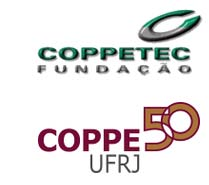
\includegraphics[width=40mm]{logo/coppetec50-logo.jpg}

\vfill%
\begin{center}
  {\GRANDE \raisebox{1.4ex}{} 
\includegraphics[width=80mm]{logo/projeto-EMMA-logo.jpg}} \\[10mm]
  %{\GRANDE \raisebox{1.4ex}{Projeto EMMA} } \\[10mm]
  {\Grande Metodologia para revestimento robótico de turbinas in situ} \\[25mm]
  {\Grande Relatório de viagem} \\[20mm]
  {\large CITENEL, Costa do Sauípe, BA} \\[5mm]
  {\large 16 a 19 de Agosto de 2015}
  \vfill%
  %{\Large \today} \\[8mm]
\end{center}

\newpage%
%---------------------------------------------------------------------
\pagestyle{fancy}%
\thispagestyle{fancy}%
\renewcommand{\headrulewidth}  {0.4pt}%
\renewcommand{\footrulewidth}  {0.4pt}%
\lhead{\vspace*{-6mm}
\includegraphics[width=30mm]{logo/lead-logo.jpg}}%
\chead{\vspace*{-6mm}\raisebox{1.7ex}{} 
\includegraphics[width=25mm]{logo/projeto-EMMA-logo.jpg}}%
%\chead{\vspace*{-6mm}\raisebox{1.7ex}{Projeto EMMA}}%
\rhead{\sf\thepage}%
\lfoot{Relatório de viagem}%
\cfoot{}%
\rfoot{\sf [\hours] \quad \today}%
%---------------------------------------------------------------------

%---------------------------------------------------------------------
%\tableofcontents

\newpage%
%---------------------------------------------------------------------
\section{Identificação}

%-----------------------------------------------------------------------
%
%   UFRJ  - Universidade Federal do Rio de Janeiro
%   COPPE - Coordenação dos Programas de Pós-graduação em Engenharia
%   PEE   - Programa de Engenharia Elétrica
%
%
%   Projeto EMMA - Metodologia para revestimento robótico de turbinas in situ
%
%   Identificação
%                                                         Ramon R. Costa
%                                                         07/jul/15, Rio
%-----------------------------------------------------------------------
%\section{Identificação}

\dado{Título}{
  EMMA - Metodologia para revestimento robótico de turbinas \textit{in situ} \\
}

\dado{Proponente}{
  Universidade Federal do Rio de Janeiro (UFRJ) \\[2mm]
  Fundação Coordenação de Projetos, Pesquisas e Estudos Tecnológicos (COPPETEC) \\
}

\dado{Contratante}{
  ESBR - Energia Sustentável do Brasil S.A. \\
}

\dado{Execução}{
  Grupo de Simulação e Controle em Automação e Robótica (GSCAR) \\
}

 \dado{Contrato}{
   Jirau 09-15 \\
 }

 \dado{P\&D ANEEL}{
   6631-0003/2015 \\
 }

%\dado{COPPETEC}{
%  N.D. \\
%}

\dado{Início}{
  26/02/2015 \\
}

\dado{Prazo}{
  14 meses \\
}

\dado{Orçamento}{
  R\$ 2.487.473,47 \\
}

\dado{Coordenador}{
  Ramon Romankevicius Costa \\
}

\dado{Gerente}{
  Breno Bellinati de Carvalho \\
}

Os engenheiros Renan Salles de Freitas e Eduardo Elael de Melo Soares
participaram do congresso e são responsáveis pela elaboração deste relatório
técnico.

%---------------------------------------------------------------------
\fim

\newpage%
%---------------------------------------------------------------------
\section{Sobre a visita}
Foram quatro dias de viagem à Costa do Sauípe, onde foi realizado o congresso
CITENEL e SEENEL:

Dia 16/08/2015:
\begin{itemize}
  \item Viagem e acomodação;
  \item Credenciamento no evento e planejamento de palestras técnicas;
\end{itemize}

Dia 17/08/2015:
\begin{itemize}
  \item Cerimônia de abertura e lançamento de revistas P\&D e EE da ANEEL;
  \item Palestra Magna - Prof. José Sidnei Colombo;
  \item Sessões técnicas;
\end{itemize}

Dia 18/08/2015:
\begin{itemize}
  \item Sessões técnicas;
\end{itemize}

Dia 19/08/2015:
\begin{itemize}
  \item Sessões técnicas;
  \item Viagem de volta;
\end{itemize}

%---------------------------------------------------------------------
\section{Considerações gerais}
A Agência Nacional de Enerngia Elétrica (ANEEL) entregou ao público a oitava
edição do Congresso de Inovação Tecnológica em Energia Elétrica (CITENEL) e a
quarta edição do Seminário de Eficiência Energética no Setor Elétrico (SEENEL),
realizados na Costa do Sauípe, Bahia, durante os dias 17, 18 e 19 de Agosto de
2015. O objetivo é ampliar a divulgação dos resultados alcançados nos
programas de Pesquisa e Desenvolvimento (P\&D) e de Eficiência Energética (EE)
regulados pela ANEEL.

A cerimônia de abertura e a palestra Magna abordaram os temas de inovação e
eficiência para o setor elétrico brasileiro, a importância da prática de
sustentabilidade, a preocupação com segurança do trabalho e primeiros socorros.

As sessões técnicas abordaram os seguintes temas: 1) redes inteligentes; 2)
planejamento de sistemas de energia elétrica; 3) geração termelétrica; 4)
eficiência energética; 5) fontes alternativas de geração de energia elétrica; 6)
supervisão, controle e proteção de sistemas de energia elétrica; 7) novos
materiais; 8) baixa renda; 9) qualidade e confiabilidade dos serviçõs de energia
elétrica; 10) medição, faturamento e combate a perdas comerciais; 11) operação
de sistemas de energia elétrica; 12) meio ambiente; 13) fontes alternativas de
geração de energia elétrica; comércio e serviços/industrial/fontes incentivadas
de energia elétrica; 14) educacional / residencial / iluminação pública; 15)
poder público; 16) segurança; 17) serviço público.

As sessões técnicas ocorriam concomitantemente, portanto foi elaborada uma
metodologia para selecionar as vinte palestras de maior interesse para o grupo. 

\section{Planejamento de sessões técnicas}
O planejamento de sessões técnicas é a metodologia criada para a seleção das
vinte palestras técnicas com maior interesse para o grupo. Como o congresso
forneceu, durante o credenciamento, todos os artigos que seriam apresentados,
foi possível selecioná-los pelo conteúdo e resultados. O grupo selecionou os
artigos que se distinguiram pela inovação tecnológica relacionados à robótica,
sensores, e sistemas que integram hardware e software no estado da arte.

Cada sessão possui 15 minutos de apresentação e 5 minutos para perguntas.

\section{Sessões técnicas}
Nesta seção, são apresentadas as principais características e aspectos técnicos
que o grupo identificou em cada sessão. As seguintes sessões técnicas foram
presenciadas:

\textbf{Desenvolvimento de veículo dubaquático para inspeção de usinas
hidrelétricas:}
Desenvolvimento de um ROV de dimensões 400x400x600 mm de fibra de vidro com
câmeras e SONAR, e um sistema de navegação com algoritmo de Monte
Carlo e validação com câmera de alta precisão. O robô assemelha-se muito ao ROV
da empresa Seabotix em sua composição mecânica, designer, sensores e distribuição de atuadores. Como o investimento
não foi alto, os atuadores não são comerciais, mas sim projetados em Solidworks
(mecânica) e Proteus (eletrônica), e montados pela própria USP, sendo capaz de
suportar correntezas de 2 m/s. O robô foi testado em usinas
hidrelétricas e foram observado ruídos eletromagnéticos na transmissão de
imagens, sendo este o desafio para a continuação do projeto.


\textbf{Robô de Inspeção de Linha -D311 :}

O palestrante apresentou o desenvolimento de um robô biomimético para inspeção
em linhas de transmissão de até 138kV. Possui sua estrutura inspirada em uma
lagarta de forma a ser capaz de atravessar obstáculos que apareçam.

O projeto foi feito com sua interface em ROS que é um framework livre. O
palestrante também ressaltou que o robô possuia avanços com relação a sua versão
anterior, como uma redução de 9kg pelo uso de titânio aeronáutico e formas ovais
para os elos, que minimizaram o ruído eletromagnético. 

Durante a sessão de perguntas o palestrante concluiu, explicando que a autonomia
do robô deverá ser expantida pelo uso de indução magnética, colhendo a energia
que passa pelo fio. Atualmente ele foi desenvolvido para ser introduzido nos
pontos de ancoragem de linha, porém o projeto para um robô de resgate já
foi desenvolvido pelo mesmo laboratório.

\textbf{Estratégias para redução da temepratura de operação de módulos
fotovoltaicos:}
Estudo de tecnologias de redução da temperatura em módulos fotovoltaicos. Foram
estudados sistemas ativos, como ventilação forçada, e sistemas passivos,  como
aletas (material de alumínio mais comum para resfriamento)
\textbf{Sistema eletrônico de captação e direcionamento de iluminação natural
para edificações utilizando fibras ópticas - girassol eletrônico:}
A motivação para a pesquisa é a baixa eficiência (5\%) de painéis FV e a
utilização da luz natural como luz para a estação de trabalho (escritório). O
sistema tem um mecanismo que rastreia o sol com um sistema Pan e Tilt e três
sensores de luz. A fibra óptica transmite a luz solar até o ambiente de trabalho
e promete eficiência de 20 a 30\%. Foram encontrados problemas em relação ao
aquecimento da fibra e duas soluções foram abordadas: solução óptica com filtros
UV e IR; e dissipador por um sistema de refrigeração com água. O último
mostrou-se mais eficiente, porém o rendimento atual observado é 5.92\% para 5 m
de fibra óptica.

\textbf{Equipamento com reconhecimento dinâmico de imagem para avaliação de
medidores de energia elétrica em campo:}

Apresentação de um equipamento medidor de consumo de energia elétrica, cujo
desenvolvimento teve duas motivações principais: verificar irregularidades na
rede elétrica, como erro de medição e precisão do medidor, e furto de rede
elétrica, conhecido popularmente como ``gato''. A principal característica do
dispositivo é sua facilidade de instalação, que pode ser realizada mesmo
com o medidor em funcionamento. São necessárias medidas de tensão, corrente e o
acoplamento de uma câmera, que filma o display de medidores digitais e tem um
algoritmo de reconhecimento para captação do giro do disco em equipamentos
analógicos.


\section{Conclusões}


%---------------------------------------------------------------------
\end{document}
